% 1977 年江苏常州市初试卷第 11 题：物体二视图——正视图（底 24 高 16 的三角形）在上，
% 俯视图（24x24 带对角线的正方形）在下，含中心线与尺寸标注（按源卷第 2 页布局）
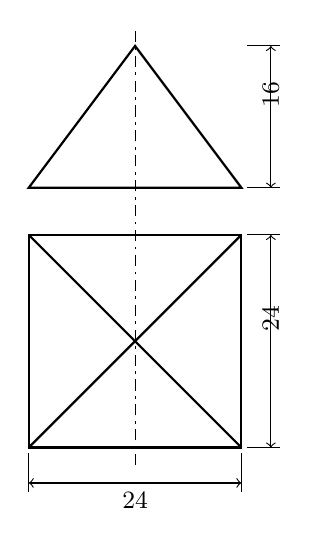
\begin{tikzpicture}[scale=0.75, font=\small]
  % 正视图：三角形
  \draw[thick] (-1.8,2.4)--(1.8,2.4)--(0,4.8)--cycle;
  % 俯视图：正方形与对角线
  \draw[thick] (-1.8,1.6)--(1.8,1.6)--(1.8,-2.0)--(-1.8,-2.0)--cycle;
  \draw[thick] (-1.8,1.6)--(1.8,-2.0);
  \draw[thick] (1.8,1.6)--(-1.8,-2.0);
  % 中心线（点划线）
  \draw[dash pattern=on 4pt off 2pt on 1pt off 2pt] (0,-2.3)--(0,5.1);
  % 尺寸标注引出线
  \draw[thin] (1.9,2.4)--(2.45,2.4);
  \draw[thin] (1.9,4.8)--(2.45,4.8);
  \draw[thin] (1.9,1.6)--(2.45,1.6);
  \draw[thin] (1.9,-2.0)--(2.45,-2.0);
  \draw[thin] (-1.8,-2.1)--(-1.8,-2.75);
  \draw[thin] (1.8,-2.1)--(1.8,-2.75);
  % 尺寸：16（正视图高）
  \draw[<->] (2.3,2.4)--(2.3,4.8) node[midway, right, rotate=90] {$16$};
  % 尺寸：24（俯视图宽）
  \draw[<->] (2.3,-2.0)--(2.3,1.6) node[midway, right, rotate=90] {$24$};
  % 尺寸：24（俯视图长）
  \draw[<->] (-1.8,-2.6)--(1.8,-2.6) node[midway, below] {$24$};
\end{tikzpicture}
